\documentclass{article}

\usepackage{titlesec}
\titleformat{\section}[block]
  {}{\S\thesection}{0.25cm}{\Large}
\title{Group Theory}
\author{Amit Rajaraman}
\date{December 2019}

\usepackage[utf8]{inputenc}
\usepackage{amsmath}
\usepackage{amssymb}
\usepackage{amsthm}
\usepackage{amsfonts}
\usepackage{enumerate}
\usepackage[margin=1in]{geometry}
\usepackage[colorlinks]{hyperref}
\usepackage{tikz}
\usepackage{titlesec}

\setlength\parindent{0pt}

\DeclareMathOperator{\Aut}{Aut}
\DeclareMathOperator{\Inn}{Inn}
\newcommand{\Mod}[1]{\ (\mathrm{mod}\ #1)}

\renewcommand{\qedsymbol}{$\blacksquare$}

\numberwithin{equation}{section}
\theoremstyle{definition}
\newtheorem{theorem}{Theorem}
\newtheorem{lemma}[theorem]{Lemma}
\newtheorem{corollary}[theorem]{Corollary}
\newtheorem{definition}{Definition}
\numberwithin{definition}{section}
\numberwithin{theorem}{section}
\newtheorem{exercise}{Exercise}
\newtheorem*{example}{Example}

\theoremstyle{remark}
\numberwithin{exercise}{section}
\newtheorem*{solution}{Solution}

\begin{document}
\maketitle
\tableofcontents
\clearpage

\section{Introduction to Groups}
    
\subsection{Definitions and Basics}

\begin{definition}
    A group $G$ is an ordered pair $(G,*)$ where $G$ is a set and $*$ is a binary operation such that
    \begin{enumerate}
        \item $(a*b)*c=a*(b*c)$ for all $a,b,c\in G$, that is, $G$ is associative.
        \item There exists an element $e$ in $G$, which we call an \textit{identity} of $G$, such that for all $g\in G$, $a*e=e*a=a$.
        \item For each $g\in G$, there exists an element $g^{-1}\in G$ called an \textit{inverse} of $g$ such that $g*g^{-1}=g^{-1}g=e$.
    \end{enumerate}
\end{definition}

We say that $G$ is a group under $*$ if $(G,*)$ is a group. If $*$ is clear from context, we sometimes just say that $G$ is a group.

We further say that $G$ is a \textit{finite group} if $G$ is a finite set. Note that any group is nonempty.

\begin{definition}
    We say that a group $(G,*)$ is \textit{abelian} if $a*b=b*a$ for all $a,b\in G$.
\end{definition}

\begin{exercise}
    Show that $\mathbb{Z}, \mathbb{R}, \mathbb{C}$ and $\mathbb{Q}$ are abelian groups under the addition operation.
\end{exercise}
\begin{exercise}
    Show that $\mathbb{Z}\setminus\{0\}, \mathbb{R}\setminus\{0\}, \mathbb{C}\setminus\{0\}$ and $\mathbb{Q}\setminus\{0\}$ are abelian groups under the multiplication operation.
\end{exercise}

We define the set $\mathbb{Z}/n\mathbb{Z}$ for some integer $n$ as follows. Let $\sim$ be an equivalence class given by
$$a\sim b\text{ if and only if }n\mid (b-a).$$
Each equivalence class is given by $\overline{a}=\{a+kn\mid k\in\mathbb{Z}\}$. There are precisely $n$ equivalence classes, namely $\overline{0}, \overline{1}, \ldots, \overline{n-1}$. These $n$ equivalence classes are the elements of the set $\mathbb{Z}/n\mathbb{Z}$.

For $\overline{a}, \overline{b}\in \mathbb{Z}/n\mathbb{Z}$, we further define addition and multiplication as
$$\overline{a}+\overline{b}=\overline{a+b}\text{ and }\overline{a}\cdot\overline{b}=\overline{a\cdot b}$$

We see that $\mathbb{Z}/n\mathbb{Z}$ is an abelian group under the addition operation with $e=\overline{0}$ and the inverse of $\overline{a}$ as $\overline{-a}$. We denote this group as $\mathbb{Z}/n\mathbb{Z}$.

Further, recall from number theory that a number $a$ has a multiplicative inverse modulo $n$ if and only if $(a,n)=1$. We also see that the set of equivalence classes $\overline{a}$ which have multiplicative inverses modulo $n$ is also an abelian group under multiplication. We denote this group as $(\mathbb{Z}/n\mathbb{Z})^\times$.


\begin{definition}
    Let $(A,\star)$ and $(B,\diamond)$ be two groups. We can form a new group $A\times B$, called the \textit{direct product} of $A$ and $B$, whose elements are those in the cartesian product, and whose operation $\cdot$ is as follows.
    $$(a_1,b_1)\cdot(a_2,b_2)=(a_1\star a_2, b_1\diamond b_2)\text{ for all }a_1,a_2\in A, b_1,b_2\in B$$
\end{definition}

\begin{theorem}
Let $G$ be a group under an operation $\star$. Then
\begin{enumerate}
    \item The identity of $G$ is unique.
    \item For each $g\in G$, $g^{-1}$ is unique.
    \item For each $g\in G$, $(g^{-1})^{-1}=g$.
    \item For any $a_1,a_2,\ldots,a_n\in G$, the value of $a_1\star a_2\star\cdots\star a_n$ is independent of how we bracket it. This is called the \textit{generalized associative law}.
    \item For $a,b\in G$, $(a\star b)^{-1}=b^{-1}\star a^{-1}$.
\end{enumerate}
\end{theorem}
\begin{proof}
We prove each of the parts of the theorem.
\begin{enumerate}
    \item Let $f$ and $g$ be two identities of $G$. We have $f\star g=f$ and $f\star g=g$, which implies that $f=g$. Thus the identity of a group is unique.
    \item Let $a,b\in G$ be two inverses of some $g\in G$. We have
    \begin{align*}
        a\star g &= b\star g\text{ where $e$ is the identity of $G$} \\
        a\star g\star a &= b\star g\star a \\
        a\star e &= b\star e \\
        a &= b
    \end{align*}
    \item We have $g^{-1}g=gg^{-1}=e$ which implies that $(g^{-1})^{-1}=g$.
    \item We leave this as an exercise to the reader. The idea is induction on $n$. First show the basis, then that any bracketing of $k$ elements $g_1,\ldots,g_k$ can be reduced to $g_1\star (g_2\star(\cdots g_k))\cdots)$. Next, argue that $a_1\star a_2\star \cdots\star a_n$ can be reduced to $(a_1\star\cdots\star a_k)\star(a_{k+1}\star\cdots\star a_n)$ for some $k$. Apply the induction condition on each subproduct to complete the result.
    \item Using the fourth result in this theorem on $(a\star b)\star(b^{-1}\star a^{-1})$ and $(b^{-1}\star a^{-1})\star (a\star b)$ gives the required result.
\end{enumerate}
\end{proof}

\textit{Notation.} Henceforth, for any group $G$ under operation $\star$, we shall write $a\star b$ as $ab$ unless it is needed that we mention it explicitly.

For some group $G$, $g\in G$ and $n\in \mathbb{Z}^+$, we write $xxx\cdots x$ ($n$ times) as $x^n$.

We usually write the identity element of any group as $1$.

\begin{theorem}
Let $G$ be a group and let $a,b\in G$. The equations $ax=b$ and $ya=b$ have unique solutions for $x,y\in G$. In particular, $ax=bx$ if and only if $a=b$ and $ya=yb$ if and only if $a=b$.
\end{theorem}
\begin{proof}
Premultiplying and postmultiplying the two equations respectively and using the fact that inverses are unique gives the unique solution for $x$ and $y$.
\end{proof}

\begin{definition}
Let $G$ be a group and $x\in G$. Let $n$ be the smallest positive integer such that $x^n=1$. This number is called the \textit{order} of $x$ and is denoted by $|x|$. If no positive power of $x$ is the identity, $x$ has order defined to be infinity and is said to be of infinite order.
\end{definition}

\begin{theorem}
\label{finGrpFinOrd}
    Any element of a finite group is of finite order.
\end{theorem}
\begin{proof}
    Let $x\in G$. There are only finitely many distinct elements among $x,x^2,x^3,\ldots$. If $x^a=x^b$ for some integers $a,b$ such that $b>a$, we have $x^{b-a}=1$, that is, $x$ is of finite order.
\end{proof}

\begin{example}
In any group, the only element of order $1$ is the identity. In the (additive) groups $\mathbb{R}, \mathbb{Z}, \mathbb{Q}$ and $\mathbb{C}$, any non-identity element is of order infinity. In $(\mathbb{Z}/7\mathbb{Z})^\times$, $\overline{2}$ is of order $3$.
\end{example}

\begin{definition}
Let $G=\{g_1,g_2,\ldots,g_n\}$ be a finite group with $g_1=1$. The \textit{multiplication table} of $G$ is an $n\times n$ matrix whose $i,j$ element is $g_ig_j$.
\end{definition}

This is a helpful way to understand the structure of any group.

\begin{definition}
Let $G$ be a group under an operation $\star$. A subset $H$ of $G$ is called a \textit{subgroup} of $G$ if $H$ also forms a group under the operation $\star$.
\end{definition}

\begin{example}
$\mathbb{Q}$ is a subgroup of $\mathbb{R}$ under addition.
\end{example}

\begin{exercise}
    If $x,g\in G$. Prove that $|x|=|gxg^{-1}|$. Deduce that $|ab|=|ba|$ for any $a,b\in G$.
\end{exercise}
\begin{exercise}
    Let $G$ be a group. Prove that if $x^2=1$ for all $x\in G$, $G$ is abelian.
\end{exercise}
\begin{exercise}
    If $x$ is an element of a group $G$, prove that $\{x^n\mid n\in\mathbb{N}\}$ is a subgroup of $G$. This subgroup is called the \textit{cyclic subgroup} generated by $x$.
\end{exercise}
\begin{exercise}
    If $x$ is an element of infinite order in $G$, prove that $x^n, n\in\mathbb{Z}$ are all distinct. Deduce that if $x^i=x^j$ for some $i,j\in\mathbb{Z}, i\neq j$, $x$ is of finite order.
\end{exercise}
\begin{exercise}
    Let $A,B$ be two groups and let $a\in A, b\in B$. Show that $(a,1)$ and $(1,b)$ commute in $A\times B$. Further show that the order of $(a,b)$ in $A\times B$ is the least common multiple of $|a|$ and $|b|$.
\end{exercise}
\begin{exercise}
    Let $G=\{1,a,b,c\}$ be a group of order $4$. If $G$ has no elements of order $4$, prove that there is a unique group table for $G$. Deduce that $G$ is abelian. This group is called the \textit{Klein four-group}.
\end{exercise}

\begin{exercise}
    Let $G$ be a group of even order. Prove that $G$ contains an element of order $2$.
\end{exercise}

\subsection{Dihedral Groups}

For each $n\in\mathbb{Z}^+$, $n\geq 3$, let $D_{2n}$ be the set of symmetries of a regular $n$-gon. A symmetry is any rigid motion of the $n$-gon which can be done by taking a copy of the polygon, moving it around in $3$-dimensional space and superimposing it on the original polygon.

We can think of this as first labeling the $n$ vertices as $1,2,\ldots,n$ and describing each symmetry of the permutation $\sigma$ of $\{1,2,\ldots,n\}$ corresponding to this symmetry.

We make $D_{2n}$ into a group by defining $st$ for $s,t\in D_{2n}$ to be the symmetry obtained by first applying $t$ then $s$. That is, if $s,t$ have corresponding permutations $\sigma$ and $\tau$, the permutation corresponding to $st$ is $\sigma\circ\tau$.

\vspace{2mm}
To find the order of $D_{2n}$, we first observe, vertex $1$ can go to any vertex $i, 1\leq i\leq n$. Next, as $2$ must remain adjacent to $1$ even after applying the symmetry, it can go to either $i+1$ or $i-1$. As we have fixed the position of two of the vertices and the polygon is rigid, we have fixed the entire permutation. We have $n\times 2=2n$ possible permutations and so, the order of $D_{2n}$ is $2n$.

\vspace{2mm}
This group is called the \textit{dihedral group of order $2n$}.

These $2n$ symmetries are the $n$ rotations by $2\pi i/n$ radians about the center for $i=1,2,\ldots,n$ and the $n$ reflections about the $n$ lines of symmetry.

\vspace{2mm}
Let $r$ be the rotation symmetry that rotates the $n$-gon by $2\pi i/n$ radians and let $s$ be the reflection symmetry that reflects the $n$-gon about the axis passing through vertex $1$ and the origin.

\begin{exercise}
    Prove the following.
    \begin{enumerate}
        \item $1,r,r^2,\ldots,r^{n-1}$ are all distinct and $r^n=1$, so $|r|=n$.
        \item $|s|=2$.
        \item $s\neq r^i$ for any $i$.
        \item $sr^i\neq sr^j$ for all $0\leq i,j\leq n-1, i\neq j$ so 
        $$D_{2n}=\{1,r,r^2,\ldots,r^{n-1},s,sr,\ldots,sr^{n-1}\}.$$
        \item $rs=sr^{-1}$.
        \item $r^is=sr^{-i}$.
    \end{enumerate}
\end{exercise}

After doing the above exercise, we observe that all the elements of $D_{2n}$ have a unique representation of the form $s^kr^i$ where $k=0\text{ or }1$ and $0\leq i\leq n-1$.

\vspace{4mm}
With the above expression of $D_{2n}$ purely in terms of $r$ and $s$ as motivation, we introduce a new concept which can help in the expression of groups in a compact way.
\begin{definition}
We say that a subset $S$ of a group $G$ is a \textit{set of generators} of $G$ if every element in $G$ can be written as a product of elements in $S$ and their inverses. We indicate this by $G=\langle S\rangle$. 
\end{definition}

For example, $\mathbb{Z}=\langle\{1\}\rangle$.

Any equations in $G$ that the generators satisfy are called \textit{relations} in $G$. So in $D_{2n}$, we have the relations $r^n=1, s^2=1$ and $rs=sr^{-1}$. It turns out that any relation in $G$ can be deduced from these three relations.

In general, if some group $G$ is generated by a set $S$ and there exist relations $R_1,R_2,\ldots,R_m$ such that any relation in $G$ can be deduced from these relations, we shall call the generators and the relations together a \textit{presentation} of $G$. We write $$G=\langle S\mid R_1, R_2,\ldots, R_m\rangle.$$

For example,
$$D_{2n}=\langle\{r,s\}\mid r^n=1, s^2=1, rs=sr^{-1}\rangle.$$

Very often, given a presentation there is some non-obvious relation that can be deduced from the given relations.

There is in fact an (as of the time of writing, unsolved) problem called the \textit{word problem} in groups, which asks for a way to determine whether two ``words" (products of elements of the group and their inverses) are equal given a set of relations.

\begin{exercise}
    Let
    $$X_{2n}=\langle\{x,y\}\mid x^n=y^2=1, xy=yx^2\rangle.$$
    Show that if $n=3k$, $X_{2n}$ has order $6$. (Note the similarity between $X_{2n}$ and $D_6$ in this case. 
    
    Also show that if $(3,n)=1$, then $x=1$.
\end{exercise}

\subsection{Symmetric groups}

Let $\Omega$ be any nonempty set and $S_\Omega$ the set of all bijections from $\Omega$ to $\Omega$ (that is, all permutations). Make $S_\Omega$ a group under function composition. (Function composition is associative, the identity is the identity mapping on $\Omega$ and any bijection has an inverse)

In the case where $\Omega=\{1,2,\ldots,n\}$, we denote $S_\Omega$ by $S_n$ and call it the \textit{symmetric group of order $n$}.

It is a simple combinatorial exercise to show that $S_n$ has exactly $n!$ elements. We now describe a notation to write the elements of $S_n$, called the \textit{cycle decomposition} of any permutation. A \textit{cycle} is a string of integers that cyclically permutes the elements of this string (leaving all other integers fixed). So the cycle $(a_1\:a_2\:a_3\:\cdots\:a_k)$ sends $a_1$ to $a_2$, $a_2$ to $a_3$, \ldots, $a_{k-1}$ to $a_k$ and $a_k$ to $a_1$. In general, for any element of $S_n$ can be rearranged and written as $k$ (disjoint) cycles as
$$\sigma=(a_1\:a_2\:\cdots\:a_{m_1})(a_{m_1+1}\:a_{m_1+2}\:\cdots\:a_{m_2})\cdots(a_{m_{k-1}+1}\:a_{m_{k-1}+2}\:\cdots\:a_{m_k})$$
This notation is very easy to read as to determine what an element $i$ is sent to, we just need to find the element written after $i$ in the cycle decomposition.

Any permutation $\sigma$ can also be easily written as its cycle decomposition using the following algorithm.
\begin{enumerate}
    \item To start a new cycle, pick the smallest number in $\{1,2,\ldots,n\}$ that has not appeared in a previous cycle. Call it $a$. Begin the new cycle $(a$.
    \item Let $\sigma(a)=b$. If $b=a$, close with a parenthesis and return to step $1$. If $b\neq a$, write $b$ next to $a$ so the cycle becomes $(a b$.
    \item Let $\sigma(b)=c$. If $c=a$, close with a parenthesis and return to step $1$. If $c\neq a$, write $c$ next to $b$ and repeat this step using $c$ as $b$ until the cycle closes.
\end{enumerate}
Naturally this process gives the correct cycle decomposition.
The \textit{length} of a cycle is the number of integers which appear in it. A cycle of length $l$ is called an $l$-cycle. We further adopt the convention that $1$-cycles are not written. (So if some $i$ does not appear in the cycle decomposition, it is understood that the permutation fixes $i$) The identity permutation is written as $1$.

So the final step in the algorithm is to remove all $1$-cycles.

\vspace{3mm}
Note that
$$(1\:3)\circ(1\:2)=(1\:2\:3)\text{ and }(1\:2)\circ(1\:3)=(1\:3\:2).$$
This shows that $S_n$ is a non-abelian group for all $n\geq 3$.

Further, since disjoint cycles permute elements in disjoint sets, disjoint cycles commute.

\begin{exercise}
    Let $\sigma=(1\:2\:\cdots\:m)$. Show that $\sigma^i$ is also an $m$-cycle if and only if $(m,i)=1$.
\end{exercise}
\begin{exercise}
    Show that the order of an $l$-cycle in $S_n$ is $l$. Deduce that the order of any element in $S_n$ is the least common multiple of the lengths of the cycles in its cycle decomposition.
\end{exercise}
\begin{exercise}
    Let $p$ be a prime. Show that an element of $S_n$ is of order $p$ if and only if its cycle decomposition is a product of commuting $p$-cycles.
\end{exercise}

\subsection{Matrix Groups}
For the sake of understanding matrix groups, we define a field as follows.

A field is a set F together with two binary operations $+$ and $\cdot$ such that $(F,+)$ is an abelian group (call its identity $0$) and $(F-\{0\},\cdot)$ is an abelian group. Further, $$a\cdot(b+c)=a\cdot b+a\cdot c\text{ for all $a,b,c\in F$}.$$

For each $n\in\mathbb{Z}^+$, we define $GL_n(F)$ to be the set of all $n\times n$ matrices whose elements are elements of F and whose determinant is nonzero. $GL_n(F)$ is a group under matrix multiplication, and is called the \textit{general linear group of order $n$}.

We have the following results (which we shall not prove in these notes).
\begin{enumerate}
    \item if $F$ is a finite field, then $|F|=p^m$ for some prime $p$ and integer $m$.
    \item if $|F|=q<\infty$, then $|GL_n(F)|=(q^n-1)(q^n-q)(q^n-q^2)\cdots(q^n-q^{n-1})$.
\end{enumerate}

\begin{exercise}
\label{defOfHeisenbergGrp}
    Let $F$ be a field. Define $$H(F)=\left\{\begin{pmatrix}1 & a & b \\ 0 & 1 & c \\ 0 & 0 & 1\end{pmatrix}\mathrel{\Bigg|} a,b,c\in F\right\}$$
    Prove that $H(F)$ is a group under matrix multiplication. This group is called the \textit{Heisenberg group} over $F$.
\end{exercise}

\subsection{Homomorphisms and Isomorphisms}
We define homomorphisms and isomorphisms here, but shall discuss them much more in detail later on.
\begin{definition}
\label{homomorphismDef}
Let $(G,\star)$ and $(H,\diamond)$ be two groups. A map $\varphi:G\to H$ such that
$$\varphi(x\star y)=\varphi(x)\diamond\varphi(y)\text{ for all $x,y\in G$}$$
is called a \textit{homomorphism}.
\end{definition}

The above condition is often compactly written as $$\varphi(xy)=\varphi(x)\varphi(y).$$

\begin{definition}
\label{defineFiberAndKer}
    Let $G,H$ be two groups and $\varphi:G\to H$ be a homomorphism. The \textit{kernel} of $\varphi$ is defined as follows.
    $$\operatorname{ker}(\varphi)=\{g\in G\mid \varphi(g)=1_H\}$$
    where $1_H$ is the identity element of $H$. The \textit{fiber} of an element $h\in H$ is defined as
    $$\varphi^{-1}(h)=\{g\in G\mid \varphi(g)=h\}.$$
\end{definition}

We see that the kernel of a homomorphism is just the fiber of the identity.

\begin{definition}
\label{isomorphismDef}
Let $G,H$ be two groups. A map $\varphi:G\to H$ is called an \textit{isomorphism} and we say $G$ and $H$ are isomorphic if $\varphi$ is a homomorphism and $\varphi$ is a bijection. If $G$ and $H$ are isomorphic, we write $G\cong H$.
\end{definition}

Intuitively, two groups being isomorphic mean that they have the same structure.

\begin{exercise}
    Show that the relation $\cong$ is an equivalence relation.
\end{exercise}

\begin{example}
    The map $f:\mathbb{R}\to\mathbb{R}^+$ given by $f(x)=e^x$ for all $x\in\mathbb{R}$ is an isomorphism from $(\mathbb{R},+)$ to $(\mathbb{R}^+,\times)$.
\end{example}

\begin{exercise}
    Let $\Omega$ and $\Delta$ be two finite sets. Show that $S_\Omega\cong S_\Delta$ if and only if $|\Omega|=|\Delta|$.
\end{exercise}

Isomorphisms are extremely useful in the study of abstract structures such as groups because if we want to study some group, it will do equally well to study a group that is isomorphic to this one.

\begin{exercise}
    Let $G$ and $H$ be two groups and $\varphi:G\to H$ be an isomorphism. Then prove that
    \begin{enumerate}
        \item if $G$ and $H$ are finite, $|G|=|H|$.
        \item $G$ is abelian if and only if $H$ is abelian.
        \item for all $x\in G$, $|x|=|\varphi(x)|$.
    \end{enumerate}
\end{exercise}

We can deduce from the third part of the above exercise that $(\mathbb{R},+)$ is not isomorphic to $(\mathbb{R},\times)$ as $-1$ is of order $2$ in $(\mathbb{R},\times)$ but there is no element of order $2$ in $(\mathbb{R},+)$.

\begin{exercise}
    Prove that $(\mathbb{R}-\{0\},\times)$ is not isomorphic to $(\mathbb{C}-\{0\},\times)$.
\end{exercise}
\begin{exercise}
    Prove that the additive groups $\mathbb{Z}$ and $\mathbb{Q}$ are not isomorphic.
\end{exercise}
\begin{exercise}
    Let $G,H$ be groups and $\varphi:G\to H$ be a homomorphism. Prove that the image of $G$ under $\varphi$ is a subgroup of $H$.
\end{exercise}

\subsection{Group Actions}
We define group actions here, but shall discuss them much more in detail later on.
\begin{definition}
    A group action of a group $G$ on a set $A$ is a map from $G\times A$ to $A$ (written as $g\cdot a$ for all $g\in G, a\in A$) such that
    \begin{enumerate}
        \item $g_1\cdot(g_2\cdot a)=(g_1g_2)\cdot a$ for all $g_1,g_2\in G, a\in A$.
        \item $1\cdot a=a$ for all $a\in A$.
    \end{enumerate}
\end{definition}

We say that $G$ is a group acting on the set $A$ in the above definition.

More precisely, this is called a \textit{left} group action. We have a similar notion of a \textit{right} group action.

\begin{theorem}
    For some fixed $g\in G$, consider the map $\sigma_g:A\to A$ given by $\sigma_g(a)=g\cdot a$. Then $\sigma_g$ is a permutation of $A$. Further, the map $G\to S_A$ given by $g\mapsto \sigma_g$ is a homomorphism.
\end{theorem}
\begin{proof}
    Consider $\sigma_{g^{-1}}:A\to A$. We shall show that $\sigma_{g^{-1}}$ is an inverse of $\sigma_g$. To see this, note that
    $$\sigma_{g^{-1}}\circ\sigma_g(a)=g^{-1}\cdot(g\cdot a)=(g^{-1}g)\cdot a=1\cdot a=a\text{ for all $g\in G$}$$
    so $\sigma_{g^{-1}}\circ\sigma_g$ is the identity map on $A$. Similarly, $\sigma_g\circ\sigma_g^{-1}$ is also the identity map on $A$. As $\sigma_g$ has a two-sided inverse, it is a bijection and thus a permutation of $A$.
    
    To see that the given map is a homomorphism, note that $$\sigma_{g_1}\circ\sigma_{g_2}(a)=g_1\cdot(g_2\cdot a)=(g_1g_2)\cdot a=\sigma_{g_1g_2}(a)\text{ for all $g_1,g_2\in G, a\in A$}.$$
    
    and $1\cdot a=a$ for all $a\in A$.
\end{proof}

\begin{definition}
\label{defKerGrpAc}
    Let a group $G$ act on a set $A$. We define the kernel of the group action as
    $$\{g\in G\mid g\cdot a=a\text{ for all }a\in A\}$$
\end{definition}

Note that any group acts on itself by the group operation itself. This action is called the \textit{left regular action} of $G$ on itself.

If a group $G$ acts on a set $A$ and distinct elements of $G$ induce distinct permutations, the action is said to be \textit{faithful}.

\clearpage
\section{Subgroups}

\subsection{Definitions and Basics}
Although we have defined subgroups in section $1$, we repeat the definition here.
\begin{definition}
Let $G$ be a group. A subset $H$ of $G$ is a subgroup of $G$ if $H$ is nonempty and it is closed under products and inverses. That is, $x,y\in H$ implies $x^{-1}\in H$ and $xy\in H$. If $H$ is a subgroup of $G$, we write $H\leq G$.
\end{definition}

If $H\leq G$ and $H\neq G$, we write $H<G$.

\begin{example}
    $\mathbb{Z}\leq\mathbb{Q}$ and $\mathbb{Q}\leq\mathbb{R}$ under the operation of addition.
    
    If $G=D_{2n}$, $H=\{1,r,r^2,\ldots,r^{n-1}\}$ is a subgroup of $G$.
\end{example}

Note that the relation $\leq$ is transitive. That is, if $K\leq H$ and $H\leq G$, then $K\leq G$.

\begin{theorem}[Subgroup Criterion]
\label{SubgroupCriterion}
A subset $H$ of a group $G$ is a subgroup if and only if
\begin{enumerate}
    \item $H\neq\emptyset$.
    \item for all $x,y\in H$, $xy^{-1}\in H$.
\end{enumerate}
Further, if $H$ is finite, then it suffices to check that $H$ is nonempty and is closed under multiplication.
\end{theorem}
\begin{proof}
    If $H\leq G$, the two given statements clearly hold as $H$ contains the identity of $G$ and is closed under inverses and multiplication.
    
    To prove the converse, let $x$ be any element of $H$ (which exists as $H\neq\emptyset$). We have $xx^{-1}\in H\implies 1\in H$. As $H$ contains $1$, for any element $h$ of $H$, $H$ contains $1h^{-1}=h^{-1}$, that is, it is closed under inverses. For any $x$ and $y$ in $H$, as $y^{-1}\in H$, we have that $x(y^{-1})^{-1}=xy\in H$, that is, $H$ is closed under multiplication.
    
    \vspace{1mm}
    To prove the second part, we see that $x,x^2,x^3,\ldots\in H$ for any $x\in H$. Using \ref{finGrpFinOrd}, we see that $x$ is of finite order $n$. Then $x^{-1}=x^{n-1}\in H$ so $H$ is closed under inverses.
\end{proof}

\begin{exercise}
    Let $G$ be a group and $H,K$ be subgroups of $G$. Show that $H\cup K$ is a subgroup if and only if $H\subseteq K$ or $K\subseteq H$.
\end{exercise}

\begin{exercise}
    Let $G$ be a group and $H,K$ be subgroups of $G$. Show that $H\cap K$ is also a subgroup of $G$.
\end{exercise}

\begin{exercise}
\label{subgrIntersubgr}
    Let $G$ be a group. Prove that the intersection of an arbitrary nonempty collection of subgroups of $G$ is again a subgroup of $G$.
\end{exercise}

\begin{exercise}
    Let $G$ be a group of order $n>2$. Show that $G$ cannot have a subgroup $H$ of order $n-1$.
\end{exercise}

\begin{exercise}
    Let $G$ be a group. Let $H=\{g\in G\mid |g|<\infty\}$. Show that $H\leq G$ if $G$ is abelian. In this case, $H$ is called the \textit{torsion subgroup} of $G$. Give an example where $G$ is non-abelian and $H$ is not a subgroup of $G$.
\end{exercise}

\begin{exercise}
    Let $H$ be a subgroup of $\mathbb{Q}$ under addition with the property that $\frac 1x\in H$ for every nonzero $x\in H$. Show that $H=\{0\}$ or $\mathbb{Q}$.
\end{exercise}

\subsection{Centralizers, Normalizers, Stabilizers and Kernels}

We now introduce some important subgroups.

\begin{definition}
    Let $G$ be a group and $A$ be any nonempty subset of $A$. Define
    $$C_G(A)=\{g\in G\mid gag^{-1}=a\text{ for all }a\in A\}.$$
    This subset is called the \textit{centralizer} of $A$ in $G$.
\end{definition}

Since $gag^{-1}=g$ if and only if $ga=ag$, $C_G(A)$ is the set of all elements that commute with every element of $A$.

Now observe that $C_G(A)$ is a subgroup of $G$ as first of all, $1\in C_G(A)$ so $C_G(A)\neq\emptyset$, and second of all, if $x,y\in C_G(A)$, we have $xax^{-1}=a$ and $yay^{-1}=a$, that is, $y^{-1}ay=a$ for all $a\in A$. We then have $a=xax^{-1}=x(y^{-1}ay)x^{-1}=(xy^{-1})a(xy^{-1})^{-1}$ so $xy^{-1}\in C_G(A)$. Thus, $C_G(A)\leq G$.

\begin{definition}
    Let $G$ be a group. Define
    $$Z(G)=\{g\in G\mid gx=xg\text{ for all }x\in G\}.$$
    This subset is called the \textit{center} of $G$.
\end{definition}

$Z(G)$ is the set of all elements that commute with every element of $G$.

As $Z(G)=C_G(G)$, we have $Z(G)\leq G$.

\begin{definition}
    Let $G$ be a group and $A$ be a subset of $G$. Define $gAg^{-1}=\{gag^{-1}\mid a\in A\}$. Define
    $$N_G(A)=\{g\in G\mid gAg^{-1}=A\}.$$
    This set is called the \textit{normalizer} of $A$ in $G$.
\end{definition}

The proof that $N_G(A)\leq G$ is similar to that we used to prove that $C_G(A)\leq G$.

Note that $C_G(A)\leq N_G(A)$.

\vspace{2mm}
If $G$ is an abelian group, $Z(G)=G$. Further, for any subset $A$ of $G$, $N_G(A)=C_G(A)=G$ as $gag^{-1}=gg^{-1}a=a$ for all $a\in A, g\in G$.

\begin{exercise}
    Show that the center of $D_8$ is $\{1,r^2\}$.
\end{exercise}

The fact that centralizers and normalizers are subgroups is in fact a special case of a results in group actions. 

We now introduce stablizers and kernels of group actions.

\begin{definition}
    Let $G$ be a group that acts on a set $S$. Let $s\in S$ be some fixed elements. Define
    $$G_s=\{g\in G\mid g\cdot s=s\}$$
\end{definition}

We shall now show that $G_s\leq G$. First of all, $1\in G_s$ by the definition of a group action. If $x,y\in G_s$, we have
\begin{align*}
    s &= 1\cdot s \\
      &= (x^{-1}x)\cdot s \\
      &= x^{-1}\cdot (x\cdot s) \\
      &= x^{-1}\cdot s
\end{align*}
so $x^{-1}\in G_s$ and
\begin{align*}
    (xy)\cdot s &= x\cdot(y\cdot s) \\
                &= x\cdot s \\
                &= s
\end{align*}
We see that $G_s$ is nonempty and is closed under inverses and multiplication. It is thus a subgroup of $G$.

Recall the definition of a \textit{kernel} of an action, \ref{defKerGrpAc}. Using \ref{subgrIntersubgr} and the fact that $G_s\leq G$ for all $s\in S$ yields the result that the kernel of any group action is a subgroup of the group.

\vspace{3mm}
We now see that $C_G(A)$ is merely the kernel of the group action of $G$ acting on $A$ as $g\cdot a= gag^{-1}$ (so it is a subgroup of $G$) and $N_G(A)$ is the stabilizer of the group action of $G$ acting on $\mathcal{P}(A)$ (the power set of $A$) as $g\cdot A=gAg^{-1}$ (so it is a subgroup of $G$).

\begin{exercise}
    Prove that $C_G(Z(G))=N_G(Z(G))=G$.
\end{exercise}

\begin{exercise}
    Prove that $H\leq N_G(H)$ for a subgroup $H$ of a group $G$.
\end{exercise}

\begin{exercise}
    For any subgroup $H$ of group $G$ and subset $A$ of $G$, define $N_H(A)=\{h\in H\mid hAh^{-1}=A\}$. Prove that $N_H(A)=N_G(A)\cap H$ and deduce that $N_H(A)\leq N_G(A)$.
\end{exercise}

\begin{exercise}
    Let $F$ be a field and the Heisenberg group $H(F)$ be defined as in \ref{defOfHeisenbergGrp}. Determine $Z(H(F))$ and prove that $Z(H(F))\cong (F,+)$.
\end{exercise}

\subsection{Cyclic Groups and Cyclic Subgroups}

\begin{definition}
    A group $H$ is \textit{cyclic} if there is some element $x\in H$ such that $H=\{x^n\mid n\in\mathbb{Z}\}$.
\end{definition}

In this case we write $H=\langle x\rangle$ and say that $H$ is \textit{generated} by $x$ and $x$ is a generator of $H$. The generator of a cyclic group need not be unique (as if $x$ is a generator, so is $-x$).

Note that any cyclic group is abelian.

\begin{example}
    The group $(\mathbb{Z},+)$ is generated by $1$ (here $1$ is the integer $1$ and not the identity).
\end{example}

\begin{theorem}
\label{orderOfCycGrpisOrderOfGen}
    Let $H=\langle x\rangle$. Then $|H|=|x|$ (where if one side of the inequality is infinite, so is the other).
\end{theorem}

\begin{proof}
    This proof is trivial and is left as an exercise to the reader.
\end{proof}

It is observed that there is a great deal of similarity between $H=\langle x\rangle$, where $|x|=n$, and $\mathbb{Z}/n\mathbb{Z}$. Both of them appear to have very similar structure. It turns out that these two groups are isomorphic, which we shall prove shortly. First, let us prove the following.

\begin{theorem}
\label{orderGCD}
    Let $G$ be an arbitrary group, $x\in G$, and let $m,n\in\mathbb{Z}$. If $x^n=1$ and $x^m=1$, then $x^d=1$, where $d=(m,n)$. In particular, if $x^m=1$ for some $m\in\mathbb{Z}$, then $|x|\mid m$.
\end{theorem}

\begin{proof}
    By the Euclidean algorithm, there exist integers $r$ and $s$ such that $d=mr+ns$. We have
    $$x^d=x^{mr+ns}=(x^m)^r(x^n)^s=1.$$
    This proves our first claim.
    
    Next, let $n=|x|$ and $x^m=1$. We have $x^d$=1, where $d=(|x|,m)$. Note that $0<d\leq |x|$ and $|x|$ is the smallest positive integer $k$ such that $x^k=1$. This implies that $d=|x|$ and $|x|=(|x|,m)$. Thus, $|x|\mid m$. 
\end{proof}

\begin{theorem}
    Any two cyclic groups of the same order are isomorphic. More specifically,
    \begin{enumerate}
        \item if $n\in\mathbb{Z}^+$ and $H=\langle x\rangle$ and $K=\langle y\rangle$ are both of order $n$, $H\cong K$.
        \item if $\langle x\rangle$ is an infinite cyclic group, $(\mathbb{Z},+)\cong\langle x\rangle$.
    \end{enumerate}
\end{theorem}
\begin{proof}
Let $\langle x\rangle$ and $\langle y\rangle$ be two cyclic groups of finite order $n$. Let $\varphi:\langle x\rangle\to\langle y\rangle$ be defined by $\phi(x^k)=y^k$. Let us first prove that $\varphi$ is well defined, that is, if $x^a=x^b$, then $\varphi(x^a)=\varphi(x^b)$. If $x^a=x^b$, $x^{b-a}=1$ and \ref{orderGCD} implies that $n\mid b-a$. Let $b=a+tn$ so
$\varphi(x^b)=\varphi(x^{a+tn})=y^{a+tn}=(y^n)^ty^a=y^a=\varphi(x^a)$. Thus $\varphi$ is well-defined. $\varphi$ is a homomorphism as $\varphi(x^a)\varphi(x^b)=y^ay^b=y^{a+b}=\varphi(x^ax^b)$. $\varphi$ is injective as any element $y^a$ of $\langle y\rangle$ is the image of $x^a$. As $\varphi$ is a surjection between two sets of equal finite order, it is a bijection and $\varphi$ is an isomorphism.

\vspace{2mm}
Let $\langle x\rangle$ be an infinite cyclic group. Consider the map $\varphi:(\mathbb{Z},+)\to\langle x\rangle$ given by $\varphi(k)=x^k$ for $k\in\mathbb{Z}$. This function is a homomorphism as $\varphi(a)\varphi(b)=x^ax^b=x^{a+b}=\varphi(a+b)$. Since $x^a\neq x^b$ for $a\neq b$, $\varphi$ is an injection. As any element $x^a\in\langle x\rangle$ is the image of $a\in\mathbb{Z}$, $\varphi$ is a surjection. Thus $\varphi$ is a bijection and an isomorphism.
\end{proof}

For each $n\in\mathbb{Z}^+$, let $\mathbb{Z}_n$ be the cyclic group of order $n$. $\mathbb{Z}_n\cong\mathbb{Z}/n\mathbb{Z}$.

\begin{theorem}
\label{orderIsOrderByGCD}
    Let $G$ be a group, $x\in G$ and $a\in\mathbb{Z}-\{0\}$.
    \begin{enumerate}
        \item If $|x|=\infty$, $|x^a|=\infty$.
        \item If $|x|=n<\infty$, $|x^a|=\frac{n}{(n,a)}$.
    \end{enumerate}
\end{theorem}

\begin{proof}
    \phantom{owo}
    \begin{enumerate}
        \item On the contrary, let $|x^a|=k<\infty$. Then $(x^a)^k=x^{ak}=1$. Also $x^{-ak}=1$. Since one of $ak$ and $-ak$ must be positive, some positive power of $x$ is $1$, which contradicts the fact that $|x|=\infty$. Thus, $|x^a|=\infty$.
        \item Let $y=x^a, d=(n,a), a=bd$ and $n=cd$ for some $b,c\in\mathbb{Z}$. We must show that $|y|=c$. We have $y^c=(x^a)^c=(x^{bd})^c=(x^{cd})^b=(x^n)^b=1$. \ref{orderGCD} implies that $|y|\mid c$. We also have $x^{a|y|}=1$ which implies that $|x|\mid a|y|$. This gives $cd\mid bd|y|$, that is, $c\mid b|y|$. However, since $(b,c)=1$, we have $c\mid |y|$. As $|y|\mid c$ and $c\mid |y|$, $|y|=c$.
    \end{enumerate}
\end{proof}

\begin{corollary}
\label{ifDivThenOrderIsDiv}
    A corollary of the second part of the above theorem is that if $a\mid n$, $|x^a|=\frac na$.
\end{corollary}

\begin{exercise}
    Assume $|x|=n<\infty$. Then $H=\langle x^a\rangle$ if and only if $(a,n)=1$.
\end{exercise}
\begin{proof}
    We have that $x^a$ generates a group of order $|x^a|$. This subgroup equals $H$ if and only if $|x^a|=|x|$, that is, $\frac{n}{(a,n)}=n$. This is equivalent to $(a,n)=1$.
\end{proof}

This implies that the total number of generators of a cyclic group of order $n$ is $\varphi(n)$, where $\varphi$ is Euler's totient function.

\begin{theorem}
    Let $H=\langle x\rangle$ be a cyclic group.
    \begin{enumerate}
        \item Every subgroup of $H$ is cyclic. More precisely, if $K\leq H$, either $K=\{1\}$ or $K=\langle x^d\rangle$, where $d$ is the smallest positive integer such that $x^d\in K$.
        \item If $|H|=\infty$, then for distinct nonnegative integers $a,b$, $\langle x^a\rangle\neq\langle x^b\rangle$. Also, $\langle x^m\rangle=\langle x^{|m|}\rangle$ so the nontrivial subgroups of $H$ are in bijection with $\mathbb{N}$.
        \item If $|H|=n<\infty$, then for each positive integer $a$ dividing $n$, there is a unique subgroup of $H$ of order $a$, namely $\langle x^{n/a}\rangle$. Furthermore, for every integer $m$, $\langle x^m\rangle=\langle x^{(n,m)}\rangle$. (So the subgroups of $H$ are in bijection with the positive integers of $n$)
    \end{enumerate}
\end{theorem}

\begin{proof}
    \phantom{beegyoshi}
    \begin{enumerate}
        \item Let $d$ be the smallest positive integer such that $x^d\in K$. As $K$ is a group, $x^kd\in K$ for any $k\in\mathbb{Z}$. Let $x^a\in K$ for some $a\in\mathbb{Z}$. Write $a=qd+r$ where $q,r\in\mathbb{Z}$ and $0\leq r<d$. Then $x^r=x^{a}x^{-qd}\in K$ as $K$ is a group. However, by the minimality of $d$ and the fact that $0\leq r<d$, we get $r=0$. As $d$ divides any $a$ such that $x^a\in K$ and $\langle x^d\rangle\leq K$, we have $K=\langle x^d\rangle$.
        \item This proof is similar to that of the third part so we leave it as an exercise to the reader.
        \item Use \ref{ifDivThenOrderIsDiv} to get that $|x^{n/a}|=a$, which gives that $\langle x^{n/a}\rangle$ is of order $a$. We must now prove that this is the unique subgroup of order $a$. Let $b\in\mathbb{Z}$ such that $\langle x^b\rangle$ is of order $a$. We have that the order of $\langle x^b\rangle$ is equal to $|x^b|$ from \ref{orderOfCycGrpisOrderOfGen}. Using \ref{orderIsOrderByGCD} gives $a=\frac{n}{(n,b)}$ so $\frac na=(n,b)$. In particular, $\frac na\mid b$. This implies that $\langle x^b\rangle\leq\langle x^\frac{n}{a}\rangle$. However, since they are of equal finite order, $\langle x^b\rangle=\langle x^\frac{n}{a}\rangle$ and $\langle x^\frac{n}{a}\rangle$ is the unique subgroup of order $a$. 
    \end{enumerate}
\end{proof}

\begin{exercise}
    Let $p$ be a prime and $n\in\mathbb{Z}^+$. Show that if $x$ is an element of a group $G$ such that $x^{p^n}=1$, then $|x|=p^m$ for some $m\leq n$.
\end{exercise}

\begin{exercise}
    Prove that $\mathbb{Z}_2\times\mathbb{Z}_2$, $\mathbb{Z}_2\times\mathbb{Z}$ and $\mathbb{Z}\times\mathbb{Z}$ are not cyclic.
\end{exercise}

\begin{exercise}
    Let $G$ be a group and $x\in G$. Prove that $g\in N_G(\langle x\rangle)$ if and only if $gxg^{-1}=x^a$ for some $a\in\mathbb{Z}$.
\end{exercise}

\begin{exercise}
    Show that $(\mathbb{Z}/2^n\mathbb{Z})^\times$ is not cyclic for any $n\geq 3$.
\end{exercise}

\subsection{Subgroups Generated by a Subset of a Group}

Throughout mathematics, there is a recurring theme wherein given an object $G$ and a subset $A$ of $G$, what is the smallest subobject of $G$ that contains $A$? For example, readers familiar with linear algebra might realize that the unique smallest subobject of a vector space that contains a given subset is just the linear span of that subset.

To make this precise in terms of groups, we can think of the minimal group as the intersection of all the subgroups that contain the given subset. This makes sense as the intersection of two subgroups is a subgroup. This was given as a question in \ref{subgrIntersubgr} but for the sake of completeness, we shall prove it here.

\begin{theorem}
\label{IntersectionOfSubgroups}
    If $\mathcal{A}$ is a nonempty collection of subgroups of a group $G$, the intersection of all members of $\mathcal{A}$ is also a subgroup of $G$.
\end{theorem}
\begin{proof}
    Let $$K=\bigcap_{H\in\mathcal{A}}H.$$
    Since $1\in H$ for every $H\in\mathcal{A}$, $1\in K$, that is, $K\neq\emptyset$. If $x,y\in K$, then $x,y\in H$ for every $H\in\mathcal{A}$. Since each $H$ is a subgroup, we have $xy^{-1}\in H$ for every $H\in\mathcal{A}$, that is, $xy^{-1}\in K$ for every $x,y\in K$. By the subgroup criterion \ref{SubgroupCriterion}, $K$ is a subgroup of $G$.
\end{proof}

We now make explicit the definition of the minimal subgroup that contains a subset.
\begin{definition}
    Let $A$ be any susbet of $G$. Define
    $$\langle A\rangle=\bigcap_{\substack{A\subseteq H \\ H\leq G}}H.$$
    This is called the \textit{subgroup of $G$ generated by $A$}.
\end{definition}

If we take $\mathcal{A}=\{H\leq H\mid A\subseteq H\}$, we see that $\langle A\rangle\in\mathcal{A}$.

We shall now try to express the subgroup generated by a subset in terms of the subset itself. Let
$$\bar{A} = \{{a_1}^{\epsilon_1}{a_2}^{\epsilon_2}\cdots{a_n}^{\epsilon_n}\mid  n\in\mathbb{Z}, n\geq0\text{ and }a_i\in A,\epsilon_i=\pm1\text{ for each }i\}.$$
and $\bar A=\{1\}$ if $A=\emptyset$. $\bar A$ is the set of all \textit{words} of elements of $A$ and their inverses.

\begin{theorem}
    Let $G$ be a group and $A$ a subset of $G$. Then $\langle A\rangle = \bar A$.
\end{theorem}
\begin{proof}
We shall first prove that $\bar A$ is a group. First of all, $\bar A\neq\emptyset$ for any $A$. If $a=a_1^{\epsilon_1}a_2^{\epsilon_2}\cdots a_n^{\epsilon_n}$ and $b=b_1^{\delta_1}b_2^{\delta_2}\cdots b_m^{\delta_m}$ are in $\bar A$, where $a,b$ are written in the same form as in the definition of $\bar A$, then $ab^{-1}=a_1^{\epsilon_1}a_2^{\epsilon_2}\cdots a_n^{\epsilon_n}b_m^{-\delta_m}b_{m-1}^{-\delta_{m-1}}\cdots b_1^{-\delta_1}\in \bar A$ as each power is still of the form $\pm 1$. \ref{SubgroupCriterion} implies that $\bar{A}$ is a subgroup.

Next, as any $a\in A$ can be written as $a^1$, $A\subseteq \bar A$ and so $\langle A\rangle\subseteq\bar A$. But as $\langle A\rangle$ is a group and is closed under inverses and multiplication, $\bar A\subseteq\langle A\rangle$. This implies that $\bar A=\langle A\rangle$.
\end{proof}

From this point on, we shall use $\langle A\rangle$ for $\bar A$. We can alternatively write $\langle A\rangle$ as
$$\langle A\rangle=\{a_1^{\alpha_1}a_2^{\alpha_2}\cdots a_n^{\alpha_n}\mid n\in\mathbb{Z}\text{ and for each }i, a_1\in A, \alpha_i\in\mathbb{Z}\text{ and }a_i\neq a_{i+1}\}$$

\begin{exercise}
    Prove that the group of positive rationals under multiplication is generated by $\{\frac 1p\mid p \text{ is a prime}\}$.
\end{exercise}

\begin{exercise}
    A group $G$ is called finitely generated if there is some finite set $A$ such that $G=\langle A\rangle$.
    \begin{enumerate}[(a)]
        \item Prove that every finitely generated subgroup of $\mathbb{Q}$ is cyclic.
        \item Prove that $\mathbb{Q}$ is not finitely generated.
    \end{enumerate}
\end{exercise}

\begin{exercise}
    A nontrivial abelian group $A$ is called \textit{divisible} if for each $a\in A$ and nonzero integer $k$, there exists $x\in A$ such that $x^k=a$.
    \begin{enumerate}[(a)]
        \item Prove that $\mathbb{Q}$ is divisible.
        \item Prove that no finite abelian group is divisible.
    \end{enumerate}
\end{exercise}

\clearpage
    
    % \textbf{\textit{Lagrange's Theorem}}:
    
    % If $G$ is a finite group and H is a subgroup of $G$, then $|H|$ divides $|G|$ and the number of left cosets of $H$ in $G$ equals $\frac{|G|}{|H|}$.
    % $\newline$
    % \textit{Proof outline}: The set of left cosets of $H$ in $G$ partition $G$. By definition of a left coset, the map $H\mapsto gH$ defined by $h\mapsto gh$ is a surjection from $H$ to the left coset $gH$. The left cancellation law implies this map is injective since $gh_1 = gh_2 \implies h_1 = h_2$. This proves that $H$ and $gH$ have the same order, $|gH|=|H|=n$.
    % Since $G$ is partitioned into $k$ disjoint subsets each of which has cardinality $n$, $|G|=kn$. Thus, $k = \frac{|G|}{|H|}$.
    
    % Note: The converse of Lagrange's Theorem (If $k\in\mathbb{Z}^{+}$ such that $k\mid|G|$, then there exists a subgroup of $G$ of order $k$) holds if $G$ is a finite abelian group.
    
    % To define a homomorphism from a group $G$ to $G'$, it is not enough to define the value of $\varphi$ at the generators of $G$, we must also ensure that the relations are satisfied. That is, if we have a relation $r=1$, where $r$ is some combination of generators, then we must also have that $\varphi (r)=1$.
    
    % Let $N$ be a subgroup of $G$. The following are equivalent:
    % \begin{enumerate}[i]
    %     \item $N \trianglelefteq G$ ($N$ is a normal subgroup of $G$)
    %     \item $N_G (N) = G$ ($N_G (N)$ is the normalizer in $G$ of $N$)
    %     \item $gN=Ng$ for all $g\in G$
    %     \item the operation of left cosets of $N$ in $G$ described by $uN\cdot vN = (uv)N$ (which is well-defined if and only if $gng^{-1}\in N$ for all $g\in G$ and all $n\in N$) makes the set of left cosets into a group.
    %     \item $gNg^{-1}\subseteq N$ for all $g\in G$ (this happens if and only if $gNg^{-1} = N$)
    %     \item $N$ is the kernel of some homomorphism.
    % \end{enumerate}
    
    % If $G = \langle S \rangle$, then if $N$ is a normal subgroup of G, $\frac GN = \langle \frac SN\rangle$.
    
    % $A\mathrel{\unlhd} B$ and $B\mathrel{\unlhd} C$ does \textit{not} imply that $A\mathrel{\unlhd} C$.
    % For example, $\langle s \rangle \mathrel{\unlhd} \langle s, r^2 \rangle \mathrel\unlhd D_8$ but $\langle s\rangle$ is not normal in $D_8$.
    
    % In abelian groups, every subgroup is normal.
    
    % If $\frac{G}{Z(G)}$ is cyclic, $G$ is abelian.
    
    % \textit{Cauchy's Theorem}: If $G$ is a finite group and $p$ is a prime dividing $|G|$, then $G$ has an element of order $p$. (Page 96 Q9, Dummit and Foote)
    
    % If $H$ and $K$ are subgroups of a group, $HK$ is a subgroup if and only if $HK=KH$.
    
    % If $H$ and $K$ are subgroups of $G$ and $H\leq N_G(K)$, then $HK$ is a subgroup of $G$. In particular, if $K\mathrel{\unlhd} G$ then $HK\leq G$ for any $H\leq G$.
    
    % Let $H\leq G$. The set of left cosets of $H$ in $G$ is in bijection with the set of right cosets of $H$ in $G$ ($x\mapsto x^{-1}$ maps each left coset to a right coset).
    
    % \begin{enumerate}
    
    % \item\textit{The First Isomorphism Theorem}: If $\varphi: G\to H$ is a homomorphism of groups, then $\ker \varphi \unlhd G$ and $G/\ker \varphi \cong \varphi(G).$
    
    % Corollary: $|G:\ker\varphi|=|\varphi(G)|$. $\varphi$ is injective if and only if $\ker \varphi = 1$.
    
    % \item\textit{The Second or Diamond Isomorphism Theorem}: Let $G$ be a group, let $H$ and $K$ be subgroups of $G$ and assume $H\leq N_{G}(K)$. Then $HK\leq G$, $K\unlhd HK$, $H\cap K\unlhd H$ and $HK/K\cong H/H\cap K$. This theorem's name can be understood from Fig. 1.
    
    % \begin{figure}[ht!]
    %     \centering
    %     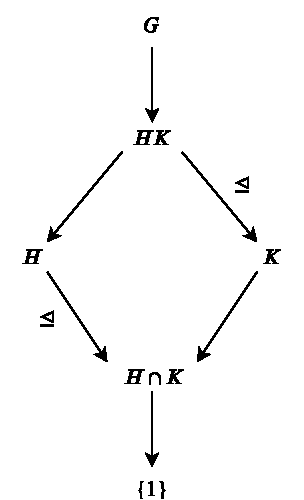
\includegraphics{img/diamondIsoThm.pdf}
    %     \caption{Diamond Isomorphism Theorem}
    %     \label{Fig. 1}
    % \end{figure}
    
    % \item\textit{The Third Isomorphism Theorem}: Let $G$ be a group and $H$ and $K$ be normal subgroups of $G$ with $H\leq K$. Then $K/H\unlhd G/H$ and $(G/H)/(K/H)\cong G/K$.
    
    % \textit{The Fourth or Lattice Isomorphism Theorem}: Let $G$ be a group and let $N$ be a normal subgroup of $G$. Then there is a bijection from the set of subgroups $A$ of $G$ which contain $N$ onto the set of subgroups $\overline{A}=A/N$ of $G/N$. In particular, every subgroup of $\overline{G}$ is of the form $A/N$ for some subgroup $A$ of $G$ containing $N$ (namely, its preimage in $G$ under the natural projection homomorphism from $G$ to $G/N$). This bijection has the following properties: for all $A,B\leq G$ with $N\leq A$ and $N\leq B$,
    % \begin{enumerate}[i]
    %     \item $A\leq B$ if and only if $\overline{A}\leq\overline{B}$,
    %     \item if $A\leq B$, then $|B\mathrel{:}A|=|\overline{B}\mathrel{:}\overline{A}|$,
    %     \item $\overline{\langle A, B\rangle} = \langle\overline{A}, \overline{B}\rangle$,
    %     \item $\overline{A\cap B}=\overline{A}\cap\overline{B}$
    %     \item $A\unlhd G$ if and only if $\overline{A}\unlhd \overline{G}$
    % \end{enumerate}
    % \end{enumerate}
    
    % If $H$ is a normal subgroup of $G$ of prime index $p$ then for all $K\leq G$, either
    % \begin{enumerate}[i]
    %     \item $K\leq H$ or
    %     \item $G=HK$ and $|K:H\cap K|=p$.
    % \end{enumerate}
    
    % In a group $G$, a sequence of subgroups $$1=N_{0} \leq N_{1} \leq N_{2} \leq\cdots\leq N_{k-1}\leq N_{k}=G$$ is called a \textit{composition series} if $N_{i} \unlhd N_{i+1}$ and $N_{i+1}/N_{i}$ is a simple group, $0\leq i\leq k-1$. If the above sequence is a composition series, the quotient groups $N_{i+1}/N_{i}$ are called \textit{composition factors} of $G$.
    
    % \textit{Jordan-H{\"o}lder Theorem:} Let $G$ be a finite group with $G\neq 1$. Then
    % \begin{enumerate}[i]
    %     \item $G$ has a composition series.
    %     \item The composition factors in a composition series are unique. Namely, if $1=N_{0} \leq N_{1} \leq N_{2} \leq\cdots\leq N_{r-1}\leq N_{r}=G$ and $1=M_{0} \leq M_{1} \leq M_{2} \leq\cdots\leq M_{s-1}\leq M_{s}=G$, then $r=s$ and there is some permutation $\pi$ of $\{1,2,\cdots, r\}$ such that $M_{\pi(i)}/M_{\pi(i)-1}\cong N_{i}/N_{i-1}$. Note that the series itself need not be unique, but the composition factors are unique.
    % \end{enumerate}    
    
    % \textit{Feit-Thompson}: If $G$ is a simple group of odd order, then $G\cong Z_p$ for some prime $p$.
    
    % A group $G$ is \textit{solvable} if there is a composition series of $G$ such that every composition factor of $G$ is abelian.
    
    % Let $G$ be a finite group. The following are equivalent:
    % \begin{enumerate}[i]
    %     \item $G$ is solvable.
    %     \item $G$ has a composition series such that every composition factor is cyclic.
    %     \item All composition factors of $G$ are of prime order.
    %     \item $G$ has a chain of subgroups: $1=N_{0} \leq N_{1} \leq N_{2} \leq\cdots\leq N_{t-1}\leq N_{t}=G$ such that each $N_i$ is a normal subgroup of $G$ and $N_{i+1}/N_{i}$ is abelian, $0\leq i\leq t-1$.
    %     \item For every divisor $n$ of $|G|$ such that $\left(n,\frac{|G|}{n}\right)=1$, $G$ has a subgroup of order $n$.
    %     \item There exists a normal subgroup $N$ of $G$ such that both $N$ and $G/N$ are solvable.
    % \end{enumerate}
    
    % The permutation $\sigma$ is odd if and only if the number of cycles of even length in its cycle decomposition is odd.
    
    % $A_n$, the alternating group of degree $n$, is a non-abelian simple group for all $n\geq5$.
    
    % An action of $G$ on $A$ may also be viewed as a faithful action of $G/\ker \varphi$ on $A$.

    % Let $G$ be a group acting on a nonempty set $A$. For each $g\in G$, the map $\sigma_{g}:A\to A$ defined by $\sigma_{g}(a)=g\cdot a$ is a permutation of $A$. There is a homomorphism associated with this action of $G$ on $A$ given as $\varphi:G\to S_A$ defined by $\varphi(g)=\sigma_{g}$ called the \textit{permutation representation} associated with this action. The kernel of this action is the same as the kernel of $\varphi$.
    
    % \begin{definition}
    % If $G$ is a group, a \textit{permutation representation} of $G$ is any homomorphism of $G$ into the symmetric group $S_A$ for some nonempty set $A$. We shall say that the given action \textit{affords} or \textit{induces} the associated permutation representation of $G$.
    % \end{definition}
    
    % Let $G$ be a group acting on the nonempty set $A$. The relation on $A$ defined by $a\sim b$ if and only if $a=g\cdot b$ for some $g\in G$ is an equivalence relation. For each $a\in A$, the number of elements in the equivalence class containing $a$ is $|G:G_a|$, where $G_a$ is the stabilizer of $a$.
    
    % Let $G$ be a group, let $H$ be a subgroup of $G$ and let $G$ act by left multiplication on the set $A$ of left cosets of $H$ in $G$. Let $\pi_H$ be the associated permutation representation afforded by this action. Then
    % \begin{enumerate}[i]
    %     \item $G$ acts transitively on $A$.
    %     \item the stabilizer in $G$ of the point $1H\in A$ is the subgroup $H$.
    %     \item the kernel of the action (i.e., the kernel of $\pi_H$) is $\cap_{x\in G}xHx^{-1}$ and $\ker\pi_H$ is the largest normal subgroup of $G$ contained in $H$.
    % \end{enumerate}
    
    % \textit{Cayley's Theorem}: If $G$ is a group of order $n$, then $G$ is isomorphic to a subgroup of $S_n$.
    
    % \textit{Proof}: Just put $H=\{1\}$ in the previous point to get a homomorphism from $G$ to $S_G$. Since the kernel is contained in $H=\{1\}$, $G$ is isomorphic to its image in $S_G$.
    
    % If $G$ is a finite group and $p$ is the smallest prime dividing $|G|$,  any subgroup of index $p$ is normal. Note that, however, a group need not necessarily have a subgroup of index $p$.
    
    % \begin{proof}
    % We have $H\leq G$ and $|G:H|=p$. Let $\pi_H$ be the permutation representation given by multiplication on the set of left cosets of $H$ in $G$. Let $K=\ker \pi_H$ and $|H:K|=k$. Then $|G:K|=|G:H||H:K|$ As there are $p$ left cosets of $H$ in $G$, we have that $G/K$ is isomorphic to a subgroup of $S_p$ (the image of $G$ under $\pi_H$). This implies $pk\mid p!$ and $k\mid (p-1)!$. The minimality of $p$ implies that $|H:K|=1$ and $H=K\unlhd G$.
    % \end{proof}
    
    % Two subsets $S$ and $T$ of $G$ are said to be conjugate in $G$ if there exists $g\in G$ such that $T=gSg^{-1}$.
    
    % The number of conjugates of a subset $S$ of $G$ is the index of the normalizer of $S$, $|G:N_G(S)|$. It follows that the number of conjugates of an element $s$ of $G$ is the index of the centralizer of $s$, $|G:C_G(s)|$. (as $N_G(\{s\})=C_G(s)$)
    
    % \textit{The Class Equation}: Let $G$ be a finite group and let $g_1, g_2, \cdots g_r$ be representatives of the distinct conjugacy classes of $G$ not contained in the center $Z(G)$ of G. Then $$|G|=|Z(G)|+\sum_{i=1}^{r}|G:C_G(g_i)|$$ Note that this is useless for abelian groups.
    
    % If $p$ is a prime and $P$ is a group of prime power order $p^{\alpha}$ for some integer $\alpha\geq 1$, then $P$ has a nontrivial center: $Z(P)\neq \{1\}$.
    
    % \begin{corollary}
    % If $|P|=p^2$ for some prime $p$, then $P$ is abelian. More precisely, $P$ is isomorphic to either $Z_{p^2}$ or $Z_p\times Z_p$.
    % \end{corollary}
    
    % Let $\tau, \sigma$ be members of the symmetric group $S_n$. Then, $\tau\sigma\tau^{-1}$ is obtained from $\sigma$ by replacing each entry $i$ in the cycle decomposition of $\sigma$ with $\tau(i)$.
    
    % If $\sigma\in S_n$ is the product of disjoint cycles of lengths $n_1,n_2,\cdots, n_r$ with $n_1\leq n_2\leq\cdots\leq n_r$ (including its $1$-cycles) then the integers $n_1,n_2,\cdots,n_r$ are called the cycle type of $\sigma$.
    
    % Two elements of $S_n$ are conjugate if and only if they have the same cycle type. The number of conjugacy classes of $S_n$ equals the number of partitions of $n$.
    
    % If $\sigma$ is an $m$-cycle in $S_n$, then $C_{S_n}(\sigma)=\{\sigma^i\tau\mid 0\leq i\leq m-1, \tau\in S_{n-m}\}$ where $S_{n-m}$ denotes the subgroup of $S_n$ which fixes the integers appearing in the $m$-cycle $\sigma$. $|C_{S_{n}}(\sigma)|=m\cdot(n-m)!$.
    
    % If $H\unlhd G$, then for every conjugacy class $\mathcal{K}$ of $G$, either $\mathcal{K}\subseteq H$ or $\mathcal{K}\cap H = \emptyset$.
    
    % If $Z(G)$ is of index $n$, any conjugacy class of $G$ is of order atmost $n$. 
    
    % Assume $H\unlhd G$, $\mathcal{K}$ is a conjugacy class of $G$ contained in $H$ and $x\in\mathcal{K}$. Then, $\mathcal{K}$ is a union of $k$ conjugacy classes of equal size in $H$, where $k = |G\mathrel{:}HC_G(x)|$.
    
    % Let $H\unlhd G$. Then $G$ acts by conjugation on $H$ as automorphisms of $H$. More specifically, the action of $G$ on $H$ by conjugation is defined for each $g\in G$ by $h\mapsto ghg^{-1}$ for each $h\in H$. For each $g\in G$, conjugation by $g$ is an automorphism of $H$. The permutation representation afforded by this action is a homomorphism of $G$ into $\operatorname{Aut}(H)$ with kernel $C_G(H)$. In particular, $G/C_G(H)$ is isomorphic to a subgroup of $\Aut(H)$.
    
    % \begin{corollary}
    % For any $H\leq G$, $N_G(H)/C_G(H)$ is isomorphic to a subgroup of $\Aut(H)$. In particular, putting $H=G$, $G/Z(G)$ is isomorphic to a subgroup of $\Aut(G)$.
    % \end{corollary}
    
    % Let $G$ be a group and $g\in G$. Conjugation by $g$ is called an \textit{inner automorphism} of $G$ and the subgroup of $\Aut(G)$ consisting of all inner automorphisms of $G$ is called $\Inn(G)$. We have that $\Inn(G)\cong G/Z(G)$ and $\Inn(G)\unlhd\Aut(G)$ ($\Aut(G)/\Inn(G)$ is called the outer isomorphism group of $G$)
    
    % $\Aut(Z_n)\cong (\mathbb{Z}/n\mathbb{Z})^{\times}$
    
    % \begin{definition}
    % A subgroup $H$ of $G$ is called \textit{characteristic} in $G$, denoted by $H \operatorname{char} G$, if every automorphism of $G$ maps $H$ to itself, i.e., $\sigma(H)=H$ for all $\sigma\in\Aut(G)$.
    % \end{definition}
    
    % Then,
    % \begin{enumerate}[i]
    %     \item characteristic subgroups are normal,
    %     \item if $H$ is the unique subgroup of $G$ of a given order, then $H \operatorname{char} G$,
    %     \item if $K\operatorname{char} H$ and $H\unlhd G$, then $K\unlhd G$ and
    %     \item if $K\operatorname{char} H$ and $H\operatorname{char} G$, then $K\operatorname{char} G$.
    % \end{enumerate}
    
    % Let $G$ be a group of order $pq$, where $p$ and $q$ are primes (not necessarily distinct) with $p\leq q$. If $p\nmid q-1$, $G$ is cyclic. The proof that $G$ is abelian is as follows.
    
    % \begin{proof}
    % If $Z(G)\neq 1$, then Lagrange's Theorem forces $G/Z(G)$ to be cyclic and hence $G$ to be abelian. Hence we may assume $Z(G)=1$.
    
    % If every nonidentity element of $G$ has order $p$, then the centralizer of every nonidentity element has index $q$, so the class equation for $G$ reads $pq = 1 + kq$. This is impossible since $q$ divides $pq$ and $kq$ but not $1$. Thus $G$ contains an element $x$ of order $q$.
    
    % Let $H=\langle x\rangle$. Since $H$ has index $p$ and $p$ is the smallest prime that divides $|G|$, $H$ is normal in $G$. Since $Z(G)=1$, we must have $C_G(H)=H$. Thus $G/H=N_G(H)/C_G(H)$ is a group of order $p$ isomorphic to a subgroup of $\Aut(H)$. But $\Aut(H)$ has order $\varphi(q)=q-1$ which by Lagrange's Theorem would imply $p\mid q-1$, contrary to the assumption.
    % \end{proof}
    
    % It can further be checked that every such group is cyclic.
    
    % Descriptions of isomorphism types of some automorphism groups:
    
    % \begin{itemize}
    %     \item The automorphism group of the cyclic group of order $p^n$ is cyclic of order $p^{n-1}(p-1)$.
    %     \item For all $n\geq 3$ the automorphism type of the cyclic group of order $2^n$ is isomorphic to $Z_{2}\times Z_{2^{n-2}}$, and in particular is not cyclic but has a cyclic subgroup of index $2$.
    %     \item Let $p$ be a prime and let $V$ be an abelian group (written additively) with the property that $pv=0$ for all $v\in V$. If $|V|=p^n$, then $V$ is an n-dimensional vector space over the field $\mathbb{F}_p=\mathbb{Z}/p\mathbb{Z}$. The automorphisms of $V$ are precisely the nonsingular linear transformations from $V$ to itself, that is, $$\Aut(V)\cong GL(V)\cong GL_n(\mathbb{F}_p).$$ In particular, the order of $\Aut(V)$ is $(p^{n}-1)(p^{n}-p)(p^{n}-p^{2})\cdots(p^n-p^{n-1})$.
    %     \item For all $n\neq 6$ we have $\Aut(S_{n})=\Inn(S_{n})\cong S_{n}$. For $n=6$, we have $|\Aut(S_{6})\mathrel{:}\Inn(S_{6})|=2$.
    %     \item $\Aut(D_8)\cong D_8$ and $\Aut(Q_8)\cong S_4$.
    % \end{itemize}
    
    % \begin{definition}
    % Let $G$ be a group and $p$ be a prime.
    % \begin{itemize}
    %     \item A group of order $p^{\alpha}$ for some $\alpha\geq 1$ is called a \textit{$p$-group}.
    %     \item If $G$ is a group of order $p^{\alpha}m$, where $p\nmid m$, then a subgroup of order $p^{\alpha}$ is called a \textit{Sylow $p$-subgroup} of $G$.
    %     \item The set of Sylow $p$-subgroups will be denote by $Syl_{p}(G)$ and the number of Sylow $p$-subgroups of $G$ will be denoted by $n_{p}(G)$ (or just $n_p$).
    % \end{itemize}
    % \end{definition}
    
    % \textit{Sylow's Theorem}: Let $G$ be a group of order $p^{\alpha}m$ where $p$ is a prime that does not divide $m$.
    % \begin{enumerate}
    %     \item Sylow $p$-subgroups of $G$ exist, i.e., $Syl_p(G)\neq\emptyset$.
    %     \item If $P$ is a Sylow $p$-subgroup of $G$ and $Q$ is any $p$-subgroup of $G$, then there exists $g\in G$ such that $Q\leq gPg^{-1}$, i.e., $Q$ is contained in some conjugate of $P$. In particular, any two Sylow $p$-subgroups of $G$ are conjugate in $G$.
    %     \item The number of Sylow $p$-subgroups of $G$ is of the form $1+kp$, i.e., $$n_p\equiv 1\Mod p.$$ Further, $n_p$ is the index in $G$ of the normalizer $N_G(P)$ for any Sylow $p$-subgroup $P$, hence $$n_p\mid m.$$
    % \end{enumerate}
    
    % Any two Sylow $p$-subgroups of a group (for the same prime $p$) are isomorphic.
    
    % Let $P\in Syl_p(G)$. If $Q$ is any $p$-subgroup of $G$, then $Q\cap N_G(P)=Q\cap P$.
    
    % Let $P$ be a Sylow $p$-subgroup of $G$. Then the following are equivalent:
    % \begin{enumerate}
    %     \item $P$ is the unique Sylow $p$-subgroup of $G$, i.e., $n_p=1$
    %     \item $P\unlhd G$
    %     \item $P\operatorname{char} G$
    %     \item All subgroups generated by elements of $p$-power order are $p$-groups, i.e., if $X$ is any subset of $G$ such that $|x|$ is a power of $p$ for all $x\in X$, then $\langle X\rangle$ is a $p$-group.
    % \end{enumerate}
    
\end{document}
